\documentclass[paper=a4,notitlepage,parskip=half,plainheadsepline]{scrartcl}

\usepackage{silence}
\WarningsOff[everypage]% Suppress warnings related to package everypage
\usepackage{snapshot} 
\usepackage{scrlayer-scrpage} 
\usepackage{iftex}
\usepackage[ngerman]{babel}
\usepackage{graphicx}
\usepackage{float}
\usepackage[T1]{fontenc}
\usepackage[utf8]{inputenc}
\usepackage{pifont}
\usepackage{amsmath}
\usepackage[german]{varioref}
\usepackage[text={6.8in,9.6in},top=0.8in,centering]{geometry}
\usepackage{datetime2}
\usepackage{array,multirow,tabularx}
\usepackage{listingsutf8}
\usepackage[table,svgnames,dvipsnames]{xcolor}
\usepackage[most,breakable,skins,listingsutf8]{tcolorbox}
%\tcbuselibrary{listingsutf8}
\usepackage[color=blue!90,scale=0.8,placement=bottom,vshift=1.2cm]{background}
\usepackage{array}
\usepackage{physics}

%%%%%%%%%%%%%%%%%%%%%%%%%%%%%%%%%%%%%%%%%%          Aufgabe oder Loesung 
\newif\ifloesung
%\loesungtrue
\loesungfalse
%%%%%%%%%%%%%%%%%%%%%%%%%%%%%%%%%%%%%%%%%%%%%%%%%%%%%%%%%%%%%%%%%%%%%%%%%


%\backgroundsetup{contents={Version vom \today}}
\backgroundsetup{contents={Version vom \today}}
%\pagestyle{empty}

\pagestyle{scrheadings}
\clearpairofpagestyles
\ihead{Fachinformatiker Anwendungsentwickler~/~Informatik--Studenten}
\chead{}
\ohead{C--Programmierung}
\ifoot{Frank Zimmermann}
\cfoot{SVLFG}
\ofoot{}
\ofoot{\pagemark}

\graphicspath{{./jpg/}}
\DeclareGraphicsExtensions{.jpg,.eps,.png}
%\usepackage{courier}


%\newcommand\bashprompt{\textcolor{cyan}{\small\ttfamily\bfseries{bob@remotehost{\textcolor{black}:}\textcolor{cyan!60}{\url{~}}{\textcolor{black}\$ }}}}
\newcommand\bashprompt{\textcolor{red!25!white}{\small\ttfamily\bfseries bash\$> }}
\newcommand\noprompt{\hspace{0.6cm}}
\newcommand{\startBash}{\gdef\myprompt{\bashprompt}}
\newcommand{\startNone}{\gdef\myprompt{\noprompt}}

\newcommand{\mingw}{\textsl{MinGW}}
\newcommand{\bash}{\emph{bash}}
\newcommand{\msys}{\textsl{MSYS}}
\newcommand{\git}{\emph{Git}}
\newcommand{\gcc}{\emph{gcc}}
\newcommand{\listingsfont}{\ttfamily}
\newcommand{\sh}{\texttt{shakespeare.c}}
\newcommand{\s}{\texttt{shakespeare}}

\RedeclareSectionCommand[
  beforeskip=-1\baselineskip,
  afterskip=.5\baselineskip]{section}
\RedeclareSectionCommand[
  beforeskip=-.75\baselineskip,
  afterskip=.5\baselineskip]{subsection}
\RedeclareSectionCommand[
  beforeskip=-.5\baselineskip,
  afterskip=.25\baselineskip]{subsubsection}
\RedeclareSectionCommand[
  beforeskip=.5\baselineskip,
  afterskip=-1em]{paragraph}
\RedeclareSectionCommand[
  beforeskip=-.5\baselineskip,
  afterskip=-1em]{subparagraph}

% Wenn pdflatex benutzt wird sollen die 
% installierten! frutiger-Fonts verwendet werden
% Ansonsten die TeX-eigenen cmbright
\ifPDFTeX %
\usepackage[scaled=0.90]{frutiger}
\renewcommand\familydefault{\sfdefault}
%\DeclareFixedFont\ott{T1}{phv}{mc}{n}{10pt
\else
\usepackage{cmbright}
\fi

\newfont{\lf}{svlfg scaled 2000}%
\newcolumntype{P}[1]{>{\centering\arraybackslash}p{#1}}

\ifloesung
\newtcbinputlisting[auto counter,list inside=lol,list type={lstlisting}]{\mylisting}[3][]{%
  toptitle=2mm,
  bottomtitle=2mm,listing only,
  colback=lightgray,
  %colback=yellow!10,
  listing file={#3},
  listing options={language=c,
  aboveskip=5pt,
  belowskip=5pt,
  columns=flexible,
  keywordstyle=\color{blue},
  basicstyle=\footnotesize\listingsfont},
  colback=white,
  %colframe=gray!75!black,
  colframe=yellow!50!black,
  listing only,
  fonttitle=\bfseries,
  breakable,
  %title={Soubor \thetcbcounter: #2},
  title=Musterlösung für \texttt{#3},
  #1
}
\fi



\begin{document}
\tcbset{enhanced,colback=green!5!white, boxrule=0.5pt, colframe=green!35!black,fonttitle=\bfseries\Large}
        % \begin{tcolorbox}[drop lifted shadow]
        % This is a tcolorbox.
        % \end{tcolorbox}\par\bigskip
        \begin{tcolorbox}[toptitle=3mm,bottomtitle=3mm,title=\centering{{\lf J}\hfil Ausbildung Fachinformatiker Anwendungsentwicklung\hfil {\lf J}},
          drop lifted shadow=gray]
        \centering{\vspace{0.5cm}\LARGE Programmierübung %
        \ifloesung (mit Musterlösung)\fi}\\[0.3cm]
        \centering{C--Programmierung / Datenstrukturen}\\\vspace{0.5cm}
        \end{tcolorbox}

\section{Aufgabe}
Es ist ein Programm (\texttt{shakespeare.c}) zu schreiben, das den Namen einer Text--Datei/Pfad
\begin{enumerate}
\item als Parameter einliest,
\item diese Datei öffnet,
\item deren Inhalt einliest,
\item bestimmte Operationen ausführt und
\item das Ergebnis in die Standard--Ausgabe schreibt.
\end{enumerate}
Der Datei/Pfadname wird als Argument für die Option \emph{-f} übergeben. Weitere optionale Parameter müssen von dem Programm eingelesen werden können. Die Parameter bestehen jeweils aus einem Buchstaben und sind durch ein vorangestelltes \texttt{-} gekennzeichnet. Diese Parameter bestimmen, wie die u.g. Operationen ausgeführt werden sollen. Beim optionalen Parameter \texttt{-h} soll lediglich eine \texttt{usage()}--Meldung ausgegeben werden (\texttt{./shakespeare [-h] [-s <n>] [-l <m>] [-f <inputfile>]}). Folgende  Parameter müssen behandelt werden können:
\begin{center}
\begin{tabular}{|P{4cm}|P{4cm}|P{7cm}|}\hline
Parameter     & Funktion          & Ausgabe\\\hline
-h            & mache garnichts   & \texttt{usage()} ausgeben\\
-f <inputfile>& Datei einlesen    & keine \\
-s  <n>       & Suchstringlänge   & default = 1 \\
-l  <n>       & Ausgabelänge      & default = Anzahl eingelesener Zeichen\\\hline
\end{tabular}
\end{center}
Das Programm soll so konzipiert werden, dass später gegebenenfalls weitere optionale Parameter leicht hinzuzufügen sind (z.B. der initiale Suchstring mit \texttt{-a <Anfang>} oder die Version mit \texttt{-v}).
Außerdem soll das Programm als \emph{Filter} arbeiten können, d.h. falls kein Datei oder Pfadname als Parameter angegeben wurde, soll das Programm seine Eingabe aus dem Kanal Standard--Eingabe (\texttt{stdin}) beziehen. Das Programm soll seine Ausgabe immer in die Standard--Ausgabe (\texttt{stdout}) schreiben.
Einige mögliche Aufrufe könnten z.B. folgendermaßen aussehen:

\newtcblisting{commandshell}{colback=black!65!white,colupper=white,colframe=black, listing only,%
listing options={style=tcblatex,language=sh,xleftmargin=0cm,breaklines=true,escapeinside={(*}{*)}},%
every listing line={\myprompt}}
%,every listing line={\textcolor{red!25!white}{\small\ttfamily\bfseries bash\$> }}
%,every listing line={\myprompt}}
\startBash
\begin{commandshell}
./shakespeare ./7zara10.txt                     
./shakespeare -s 3 -l 1000 ./7zara10.txt                
./shakespeare -s5 -l500 ./7zara10.txt                   
./shakespeare -s 8 -f ./7zara10.txt         
./shakespeare  -h                           
cat ./7zara10.txt | ./shakespeare -s 8   
./shakespeare -s4 -l1000 < ./7zara10.txt     
\end{commandshell}

Zum Programm soll eine etwa 4--seitige Dokumentation erstellt werden, in der die Arbeitsweise und der Aufbau des Programms kurz skizziert wird. Dabei sollte auch auf die verwendeten Datenstrukturen eingegangen werden.

Eine mögliche Ausgabe (der anfängliche Suchstring steht in spitzen Klammern) könnte ungefähr so aussehen:

\begin{commandshell}
(*\startBash*)./shakespeare -s6 -l400 ./7zara10.txt(*\startNone*)
<Friedr>ich Nichts; du so langsam, was auf deinem Auge. Dass du mir und Klapper mit Vorsicht. Aber ein Dichternen wie sieben dem als an Hoefen? Ein Arzt? Oder boese Blick _aller_ Dinge sie, die sich "die Lust. Lust nannte keine Gipfel zu neuen Frevelhaften Vortheil." Ungerechtig auf und hinweg und rauchten sie mich selber abwendet. Diess nach Vater, antwortete der Erde an und Grauen wissen auch deinetwill(*\startBash*)
./shakespeare -s6 -l400 ./7zara10.txt(*\startNone*)
<Friedr>ich Nichts lebt nicht es mir fragt der wieder und Entsagung. Sonderlich. Kein Hunger. Oft kommt er mir, so will es seiner Kuh: welche wieder _hoffende. Und wer werde vor Maechtigen: `Ja, ich mit _meine_ Sonnen-Pfeile, ein faulichkeit die den letzten Stuhl in die Wahrsager und tanzen macht mir dieser Vogels. Aber sein - und ich hart an seinem Hausthiere mieden, eine Mittel zu Ende zum(*\startBash*)
./shakespeare -s11 -l400 ./7zara10.txt(*\startNone*)
<Friedrich N>ietzsche
Also sprach Zarathustra von der Stelle hin, woher die Stimme kam, und sahen zu ihm hinauf. Solchergestalt waren sie Alle: ihr Wahnsinn in der Liebe.
Licht bin ich: ach, dass die Macht gnaedig wird und herabkommt in's Sichtbare: Schoenheit waechst, was Einer mit seinem Blute, Zarathustra; noch nahmst du meinen Dank nicht an! Ward meine Welt nicht eben vollkommener als einem Vater, am aehn    
\end{commandshell}
\section{Funktionen der Parameter}
Das Programm soll einen neuen Zufallstext ausgeben, der aus dem eingelesenen Text folgendermaßen berechnet wird:

\begin{description}
\item[-s <n>] Mit diesem Parameter wird die Suchstringlänge angegeben. Es wird nach einem Suchstring dieser angegebenen Länge im eingelesenen Text gesucht. Zuvor wird ein String dieser Länge aus dem eingelesenen Text ausgewählt (die ersten Zeichen). Dieser String ist dann der \emph{Suchstring}.

Dann wird dieser String im gesamten Text gesucht. Der Folgebuchstabe hinter diesem String wird sich gemerkt und für jeden gefundenden Folgebuchstabe wird gezählt, wie oft er hinter diesem Suchstring im Text vorkommt. Dann wird hinter den Suchstring ein neuer Folgebuchstabe angehängt, der aus der Menge aller gefundenen Folgebuchstabe zufällig, aber unter Berücksichtigung der Wahrscheinlichkeit des Vorkommens, ausgewählt wird. 

Anschließend wird bei dem um ein Zeichen verlängerte Suchstring das erste Zeichen nicht beachtet. Der neue Suchstring mit dem angefügten Zeichen hinten und dem vernachlässigten Zeichen vorne hat dann die gleiche Länge wie der anfängliche Suchstring. Mit diesem neuen Suchstring wird das Verfahren wiederholt.

Damit lässt sich ein neuer Ausgabestring erzeugen, der einen Zufallstext erzeugt, der sich aus dem eingelesenen Text zufällig ergibt.

Je kürzer der Suchstring ist, desto unsinniger wird der ausgegebene Text sein. Bei einer Länge von mehr als 5 Zeichen werden schon oft ganze Wörter berücksichtigt und der vermeintliche Sinn des ausgegebenen Textes erscheint mehr und mehr vorhanden.
Ein Beispiel für eine Suchstringlänge von 5 ($\langle abcde \rangle$) würde folgendermaßen aussehen: 
\begin{equation*}
\langle abcde \rangle_1 + [x_1]  \Rightarrow\ \langle bcdex_1 \rangle_2 + [x_{2}]  \Rightarrow\ \langle cdex_1x_2 \rangle_3 + [x_{3}] \ldots  
\end{equation*}
Dabei ist $[x_i]$ jeweils ein aus der Wahrscheinlichkeitsverteilung gewählte Buchstabe, der als Folgebuchstabe zum aktuellen Suchstring $\langle \ldots \rangle_i$ im gesamten Text gefunden wurde.
\item[-l <n>] Mit diesem Parameter wird die Anzahl der Zeichen angegeben, die vom Programm ausgegeben werden sollen. Der \emph{default}--Wert ist der gesamte Eingabetext. Falls dieser aber sehr groß ist und man nur einen Text begrenzter Länge benötigt, kann man mit diesem Parameter die Länge angeben. Der Parameter muß aber nicht unbedingt die Ausgabe begrenzen, er kann sie auch erweitern, da der generierte Text ja zufällig gebildet wird
(eine Begrenzug des auszugebenden Textes sollte durch die vom Compiler größte maximal darstellbare Integer--Zahl erfolgen).

\end{description}

\section{Bemerkungen und Tips}
Die Entwicklungsumgebung ist \mingw. Getestet wird das Programm am günstigsten in einer \git--\bash.

Das Einlesen der Parameter, Datei und die Verwendung als Filter sollte keine Probleme darstellen.

Eine Herausforderung stellt die Erarbeitung des Algorithmus mit den dazugehörigen Datenstrukturen dar. Daher ist es vorteilhaft, erst das Gerüst zur Behandlung der Parameter und das Einlesen der Textdatei auszuprogrammieren und zu testen.

Anschließend versuchen Sie einen Algorithmus und eine Datenstruktur zu finden, die die Anforderungen erfüllen. Bei allen Überlegungen sollte auch immer der benötigte Speicherplatz und die Laufzeit des Programmes im Auge behalten werden.
Nutzen Sie Ihr Wissen über Datenstrukturen, um einen effektiven Algorithmus zu finden. Hier muss nicht nur programmiert werden, sondern es muss auch ein Konzept, die Datenstruktur und ein Algorithmus geplant werden.

Testen Sie mit einer überschaubaren kleinen Eingabedatei, bei der sich die Ausgabe leicht überprüfen lässt.

Fassen Sie die nur für die Datenstrukturen benötigten Hilfsprogramme und Datenstrukturen in externen Dateien zusammen, um die Übersicht zu behalten (Modularisierung). Da diese Aufgabe ein wenig komplexer als die vorherige ist, empfiehlt es sich hier besonders, einzelne Funktions--Komponenten gut gegeneinander abzugrenzen und separat zu testen. Nutzen Sie selbst erstellte Skizzen und Programmablaufpläne. Ein Programmieren \emph{aus dem Bauch heraus} könnte leicht zu einem Durcheinander führen.

\section{Hintergrundinformationen}
Das Problem gehört zu einer Klasse von Problemen, bei dem ein Zustand durch einen festen Algorithmus immer wieder in einen neuen Zustand überführt wird. Die Menge der möglichen Zustände ist dabei fest.

Konkret ist hier die Menge der möglichen Zustände die Menge aller Möglichkeiten, einen String in der Länge des Suchstrings zu erzeugen. Bei einer Alphabetgröße z.B. von $50$ ist die
 $$(\text{Menge aller möglichen Zustände für einen String der Länge } s) =  50^s$$. 

Mathematisch läßt sich so ein Problem durch einen sogenannten \emph{Markov--Prozeß} (\emph{Markov--Kette}) beschreiben.
Dabei wird aus einem Zustandsvektor (geordnete Menge aller möglichen Zustände: $V_i^{\mathrm{alt}}$) durch Multiplikation mit einer Übergangsmatrix (enthält die Wahrscheinlichkeiten für die einzelnen Übergänge: $P_{ij}$) ein neuer Zustandsvektor ($V_i^{\mathrm{neu}}$) erzeugt.) (

$$V^\mathrm{neu}_j = P_{ij} * V^\mathrm{alt}_i$$

Für dieses konkrete Problem sähen die Zustandsvektoren für einen 3--stelligen Suchstring etwa so aus:


$$V_i = \left( \begin{array}{c}P(AAA)\\P(AAB)\\P(ABA)\\\dots\\P(DER)\\\dots \end{array}\right) 
      = \left(\begin{array}{c}0\\0\\0\\\dots\\1\\\dots \end{array}\right)$$ 

Aus diesem Zustandsvektor geht dann mit gewissen Wahrscheinlichkeiten ein neuer Zustandsvektor hervor. Die Wahrscheinlichkeiten sind durch die Häufigkeiten der Folgebuchstaben für den jeweiligen String definiert.


\begin{minipage}[t]{0.5\textwidth}
\vspace{0pt}
Der Index des Zustandsvektors kennzeichnet also den konkreten String. Steht dort bei $V^\mathrm{alt}$ eine 1, so ist dieser String gerade der aktuelle Suchstring. Aus diesem Zustandsvektor wird ein neuer Zustandsvektor, der bei maximal 50 Indizes (weil nur 50 verschiedene neue Buchstaben angehängt werden können) jeweils eine Zahl zwischen 0 und 1 besitzt. Diese Zahl repräsentiert die Wahrscheinlichkeit für die Wahl dieses Strings als den neuen Suchstring (alle Zahlen müssen sich daher zu 1 addieren). Mit diesen Wahrscheinlichkeiten wird ein neuer Suchstring ausgewählt (dort erscheint jetzt eine 1 und alle anderen Zeilen im Zustandsvektor werden zu 0) und der Prozess wiederholt sich. Dabei bleibt die Übergangsmatrix dieselbe, da sie nur von dem Originaltext abhängt.

Damit wäre der Algorithmus zumindest theoretisch vorgegeben.
\end{minipage}
\hfill
\begin{minipage}[t]{0.5\textwidth}
\vspace{0pt}
\centering

\includegraphics[width=1\textwidth]{FuerAufgabe02.png}
\end{minipage}

Man müsste nur die Matrix für die Übergangswahrscheinlichkeiten aus dem Text errechnen und dann für jeden neuen Zufallsbuchstaben die Matrix mit dem Zustandsvektor multiplizieren. Dann erhält man einen neuen String mit den zugeordneten Wahrscheinlichkeiten und wählt einen gemäß der Wahrscheinlichkeit aus.

Praktisch ist das aber so nicht möglich da:
\begin{itemize}
\item Bei einer etwas größeren Länge für den Suchstring (wo es interessant wird: $s>5$) wird der Zufallsvektor sehr groß. Für $s=5$ und einem 50--Zeichen-Alphabet ergibt sich eine Zustandsanzahl von 312500000.
Eine Suchstringlänge von 10 ergibt z.B. schon eine Zustandsanzahl von 97656250000000000.
\item Der Zustandsvektor enthält bei einem 50--Zeichen--Alphabet nur maximal 50 Einträge ungleich Null. Damit besteht er fast nur aus Nullen.
\item Die Übergangsmatrix, die die Wahrscheinlichkeiten enthält ist von der Größe des Quadrats der Größe der Zustandsvektoren und entsprechend groß.
\item Abgesehen von dem astronomisch hohen Speicherbedarf würde die Berechnung bei diesen Größen entsprechend lange dauern. 
\item Wird der Suchstring um ein Zeichen erhöht, so würde der Speicherbedarf für den Zustandsvektor um den Faktor 50 wachsen und der Speicherbedarf für die Übergangsmatrix um den Faktor $50*50=2500$. Man sagt hier, dass der Algorithmus schlecht mit der Eingangsgröße \emph{skaliert} (exponentiell). Dies wird mit der sogenannten \emph{O--Notation} ausgedrückt, die angibt in welcher Stärke der Speicherbedarf bzw. die Laufzeit mit der Eingangsgröße wächst. Hier hätten wir ein exponentielles Ansteigen: $O(k^n),k>2$).
Für Algorithmen strebt man (abgesehen von $O(1)$) eine Komplexität von $O(log(n))$ oder $O(n)$, schlimmstenfalls $O(n^2)$ an. 
\end{itemize} 

Obwohl wir hier eigentlich einen klaren Algorithmus hätten , der einfach ausprogrammiert werden könnte (und auf 1-- und 2--dimensionalen Feldern/Arrays beruht), müssen wir nach einem praktischeren Algorithmus suchen, der mit dem zur Verfügung stehenden Speicher auskommt und ihn effizienter nutzt!

%\section{Bewertung}
%Die Programme werden ausgeführt (als Filter oder als Einzelapplikation) und müssen eine grössere Datei verarbeiten. Dabei wird die Richtigkeit der Ausgabe (50\%) und die Geschwindigkeit der Verarbeitung (25\%) gemessen. Weiterhin wird die Dokumentation und Strukturierung mit 25\% bewertet.

\section{Abgabe} 
Die lauffähigen Programme und der kommentierte Quelltext sind mit einer etwa 4--seitigen Dokumentation abzugeben (Email, Dokumentation in HTML,\TeX\  oder \texttt{ASCII}). %Abgabetermin ist der 13.11.2020.

\section{Zeitrahmen}
Der Zeitrahmen dieser Aufgabe ist mit etwa 60 Stunden angesetzt.

\ifloesung
\newpage
\section{Musterlösung}
Der Programmablaufplan:

\begin{center}
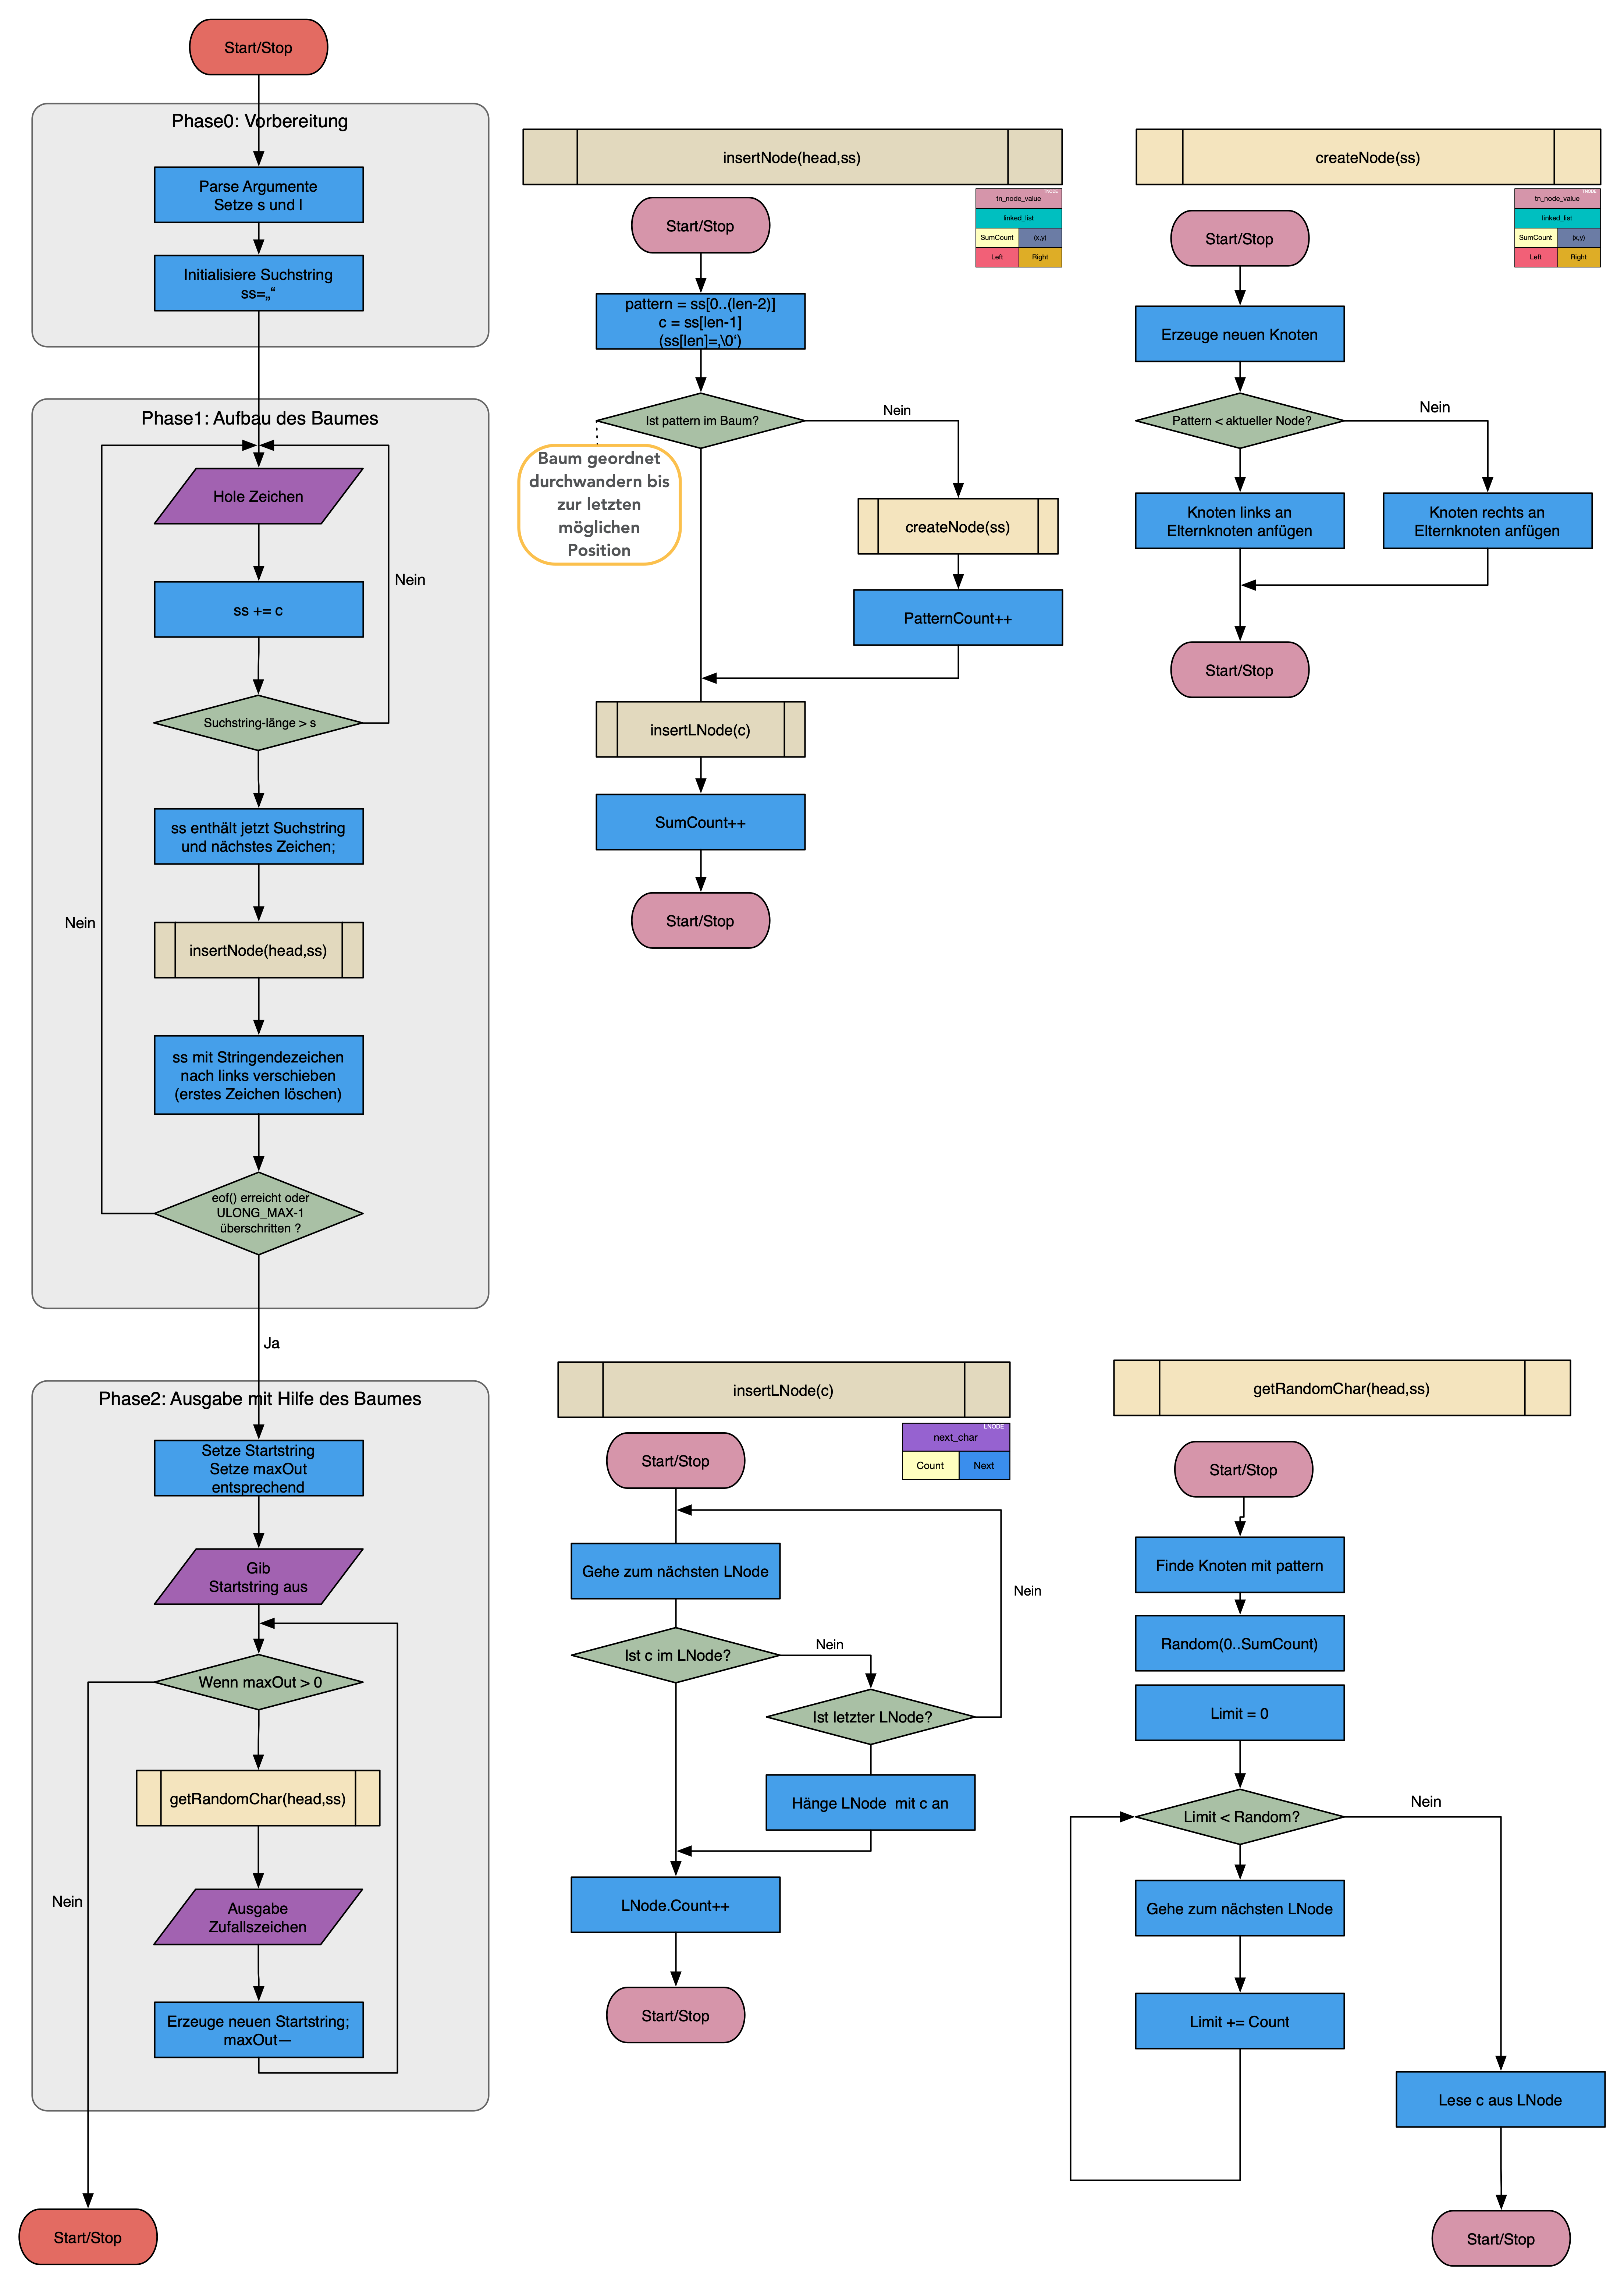
\includegraphics[width=0.90\textwidth]{Aufgabe02Flowchart}
\end{center}
\newpage
Die Datenstruktur zum Abspeichern der eingelesenen Information und der Generierung des Zufallstextes:

\begin{center}
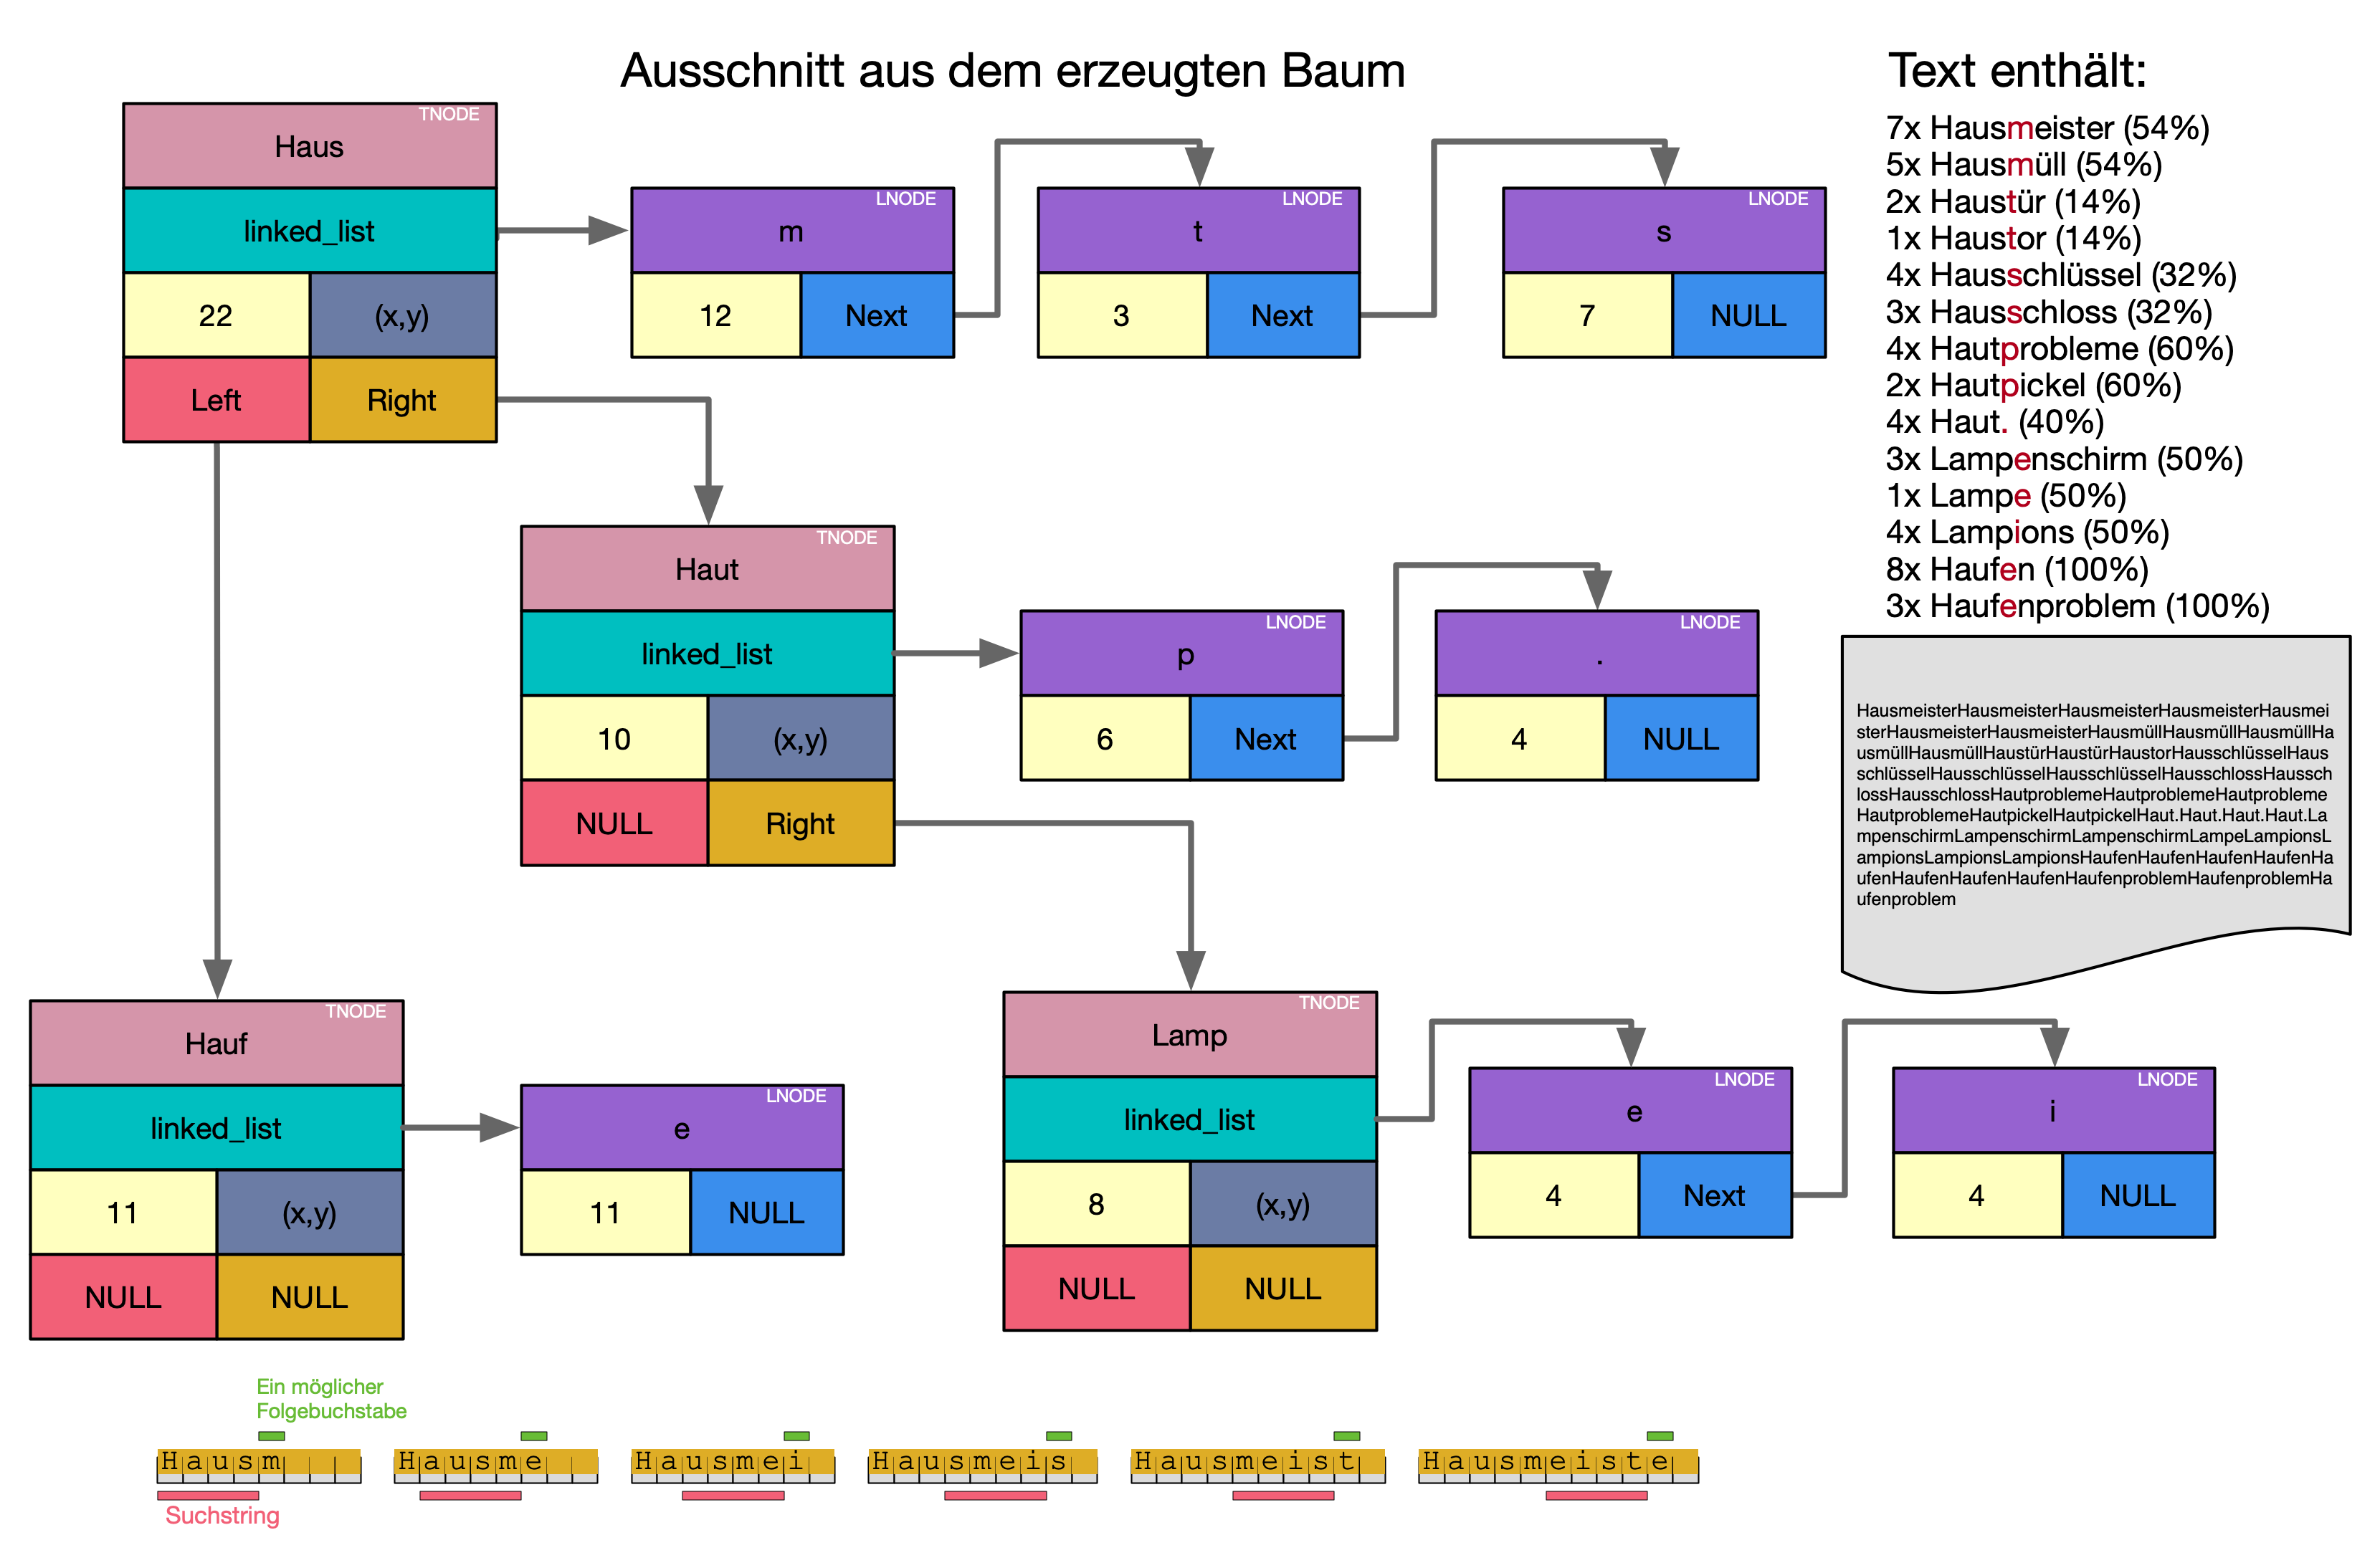
\includegraphics[width=\textwidth]{shakespeareDatenstruktur.png}
\end{center}

\lstset{ % General setup for the package
%     language={C},
%     basicstyle=\small\sffamily,
     numbers=left,
     numberstyle=\tiny,
%     frame=tb,
%     tabsize=4,
%     columns=flexible,
     showstringspaces=true,
     numbersep=5pt,
%     showtabs=false,
%     keepspaces,
     commentstyle=\color{olive},
     inputencoding=utf8/latin1
%     keywordstyle=\color{blue}
}%

\newpage
Die Auswahl des zufällig bestimmten Buchstabens aus den gewichteten Wahrscheinlichkeiten kann folgendermaßen erfolgen:
\begin{center}
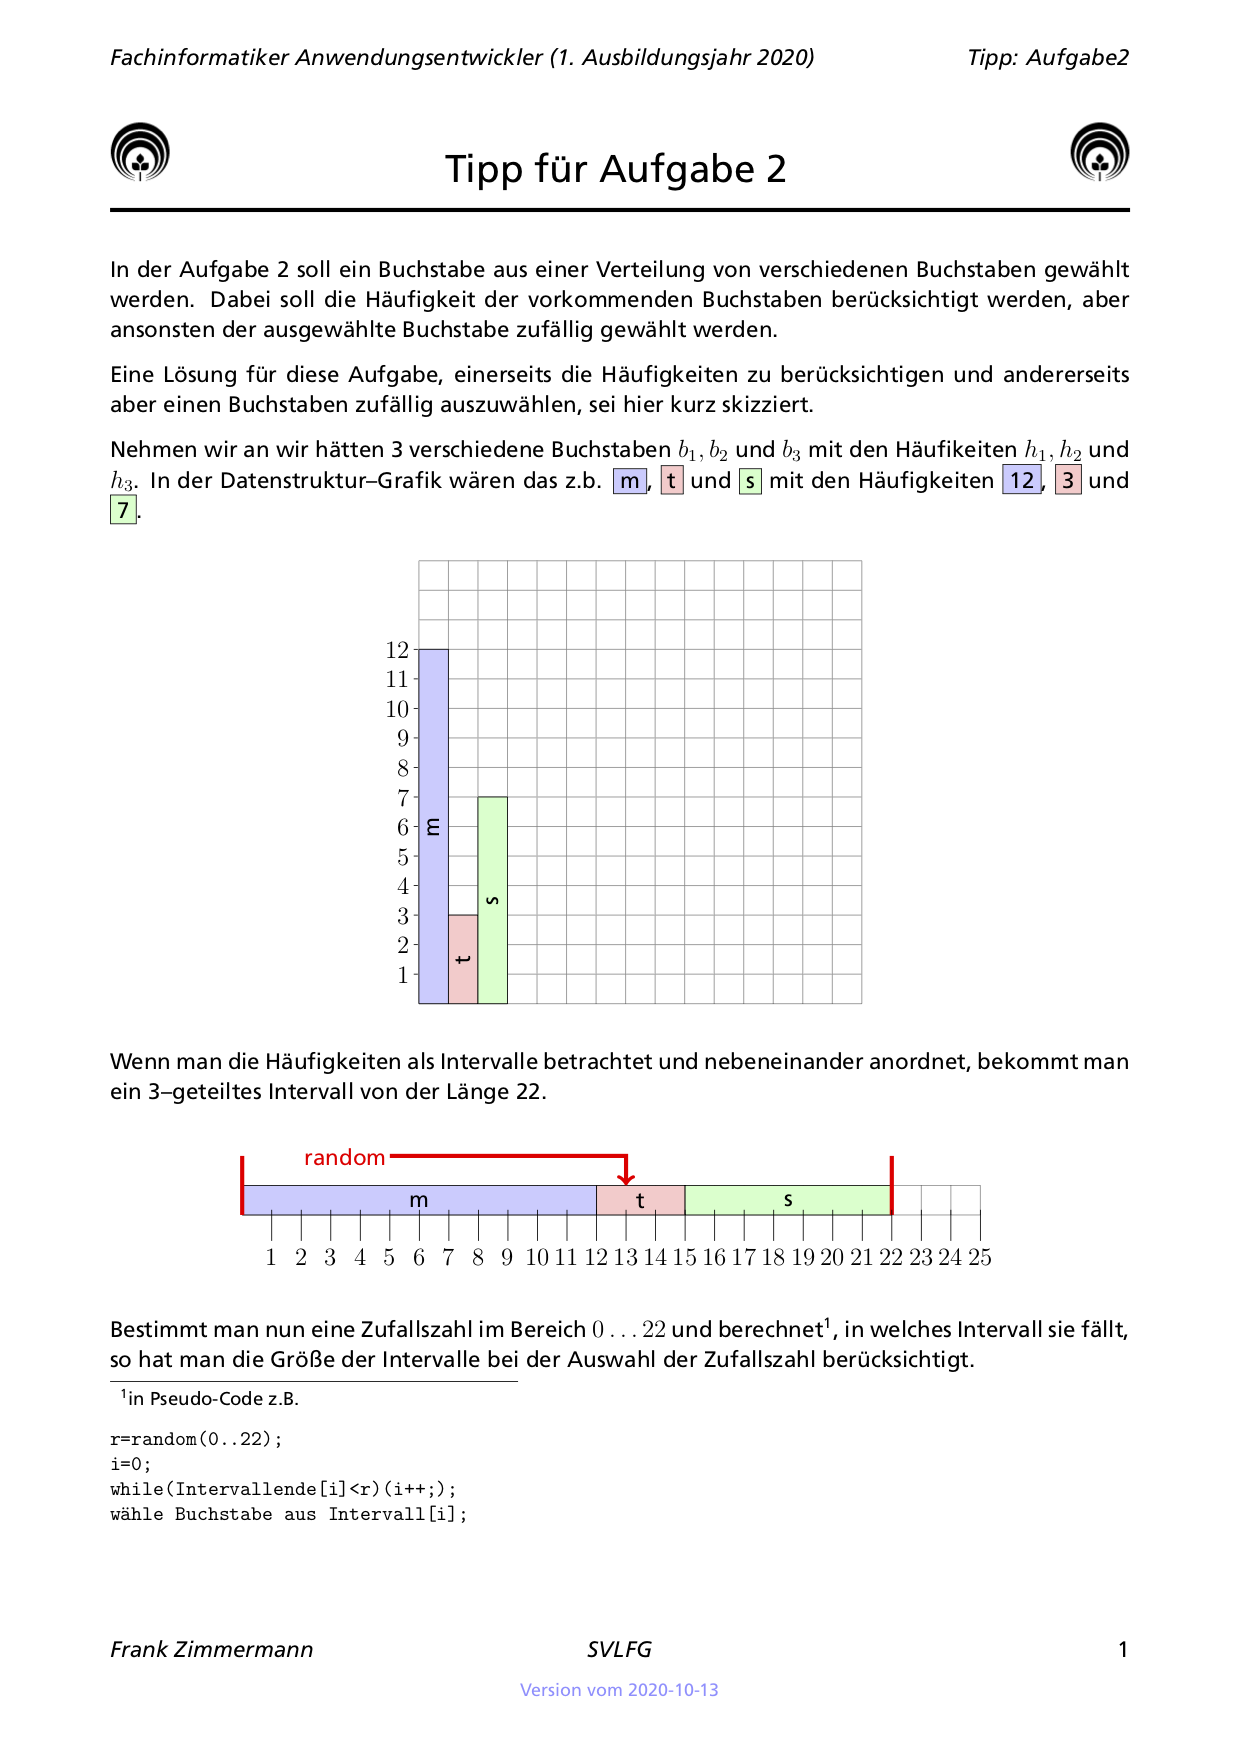
\includegraphics[width=0.93\textwidth]{TippWahrscheinlichkeiten.png}
\end{center}
\newpage
Die Musterlösung enthält auch einen optionalen Parameter \texttt{-d} für das Programm, der nicht gefordert wurde aber zur leichteren Übersicht mit in die Musterlösung eingebaut wurde. Der Schalter \texttt{-d7} druckt den erstellten Baum (hier mit \texttt{-s2}) u.a. auch als Baumstruktur im PostScript--Format. 
\begin{center}
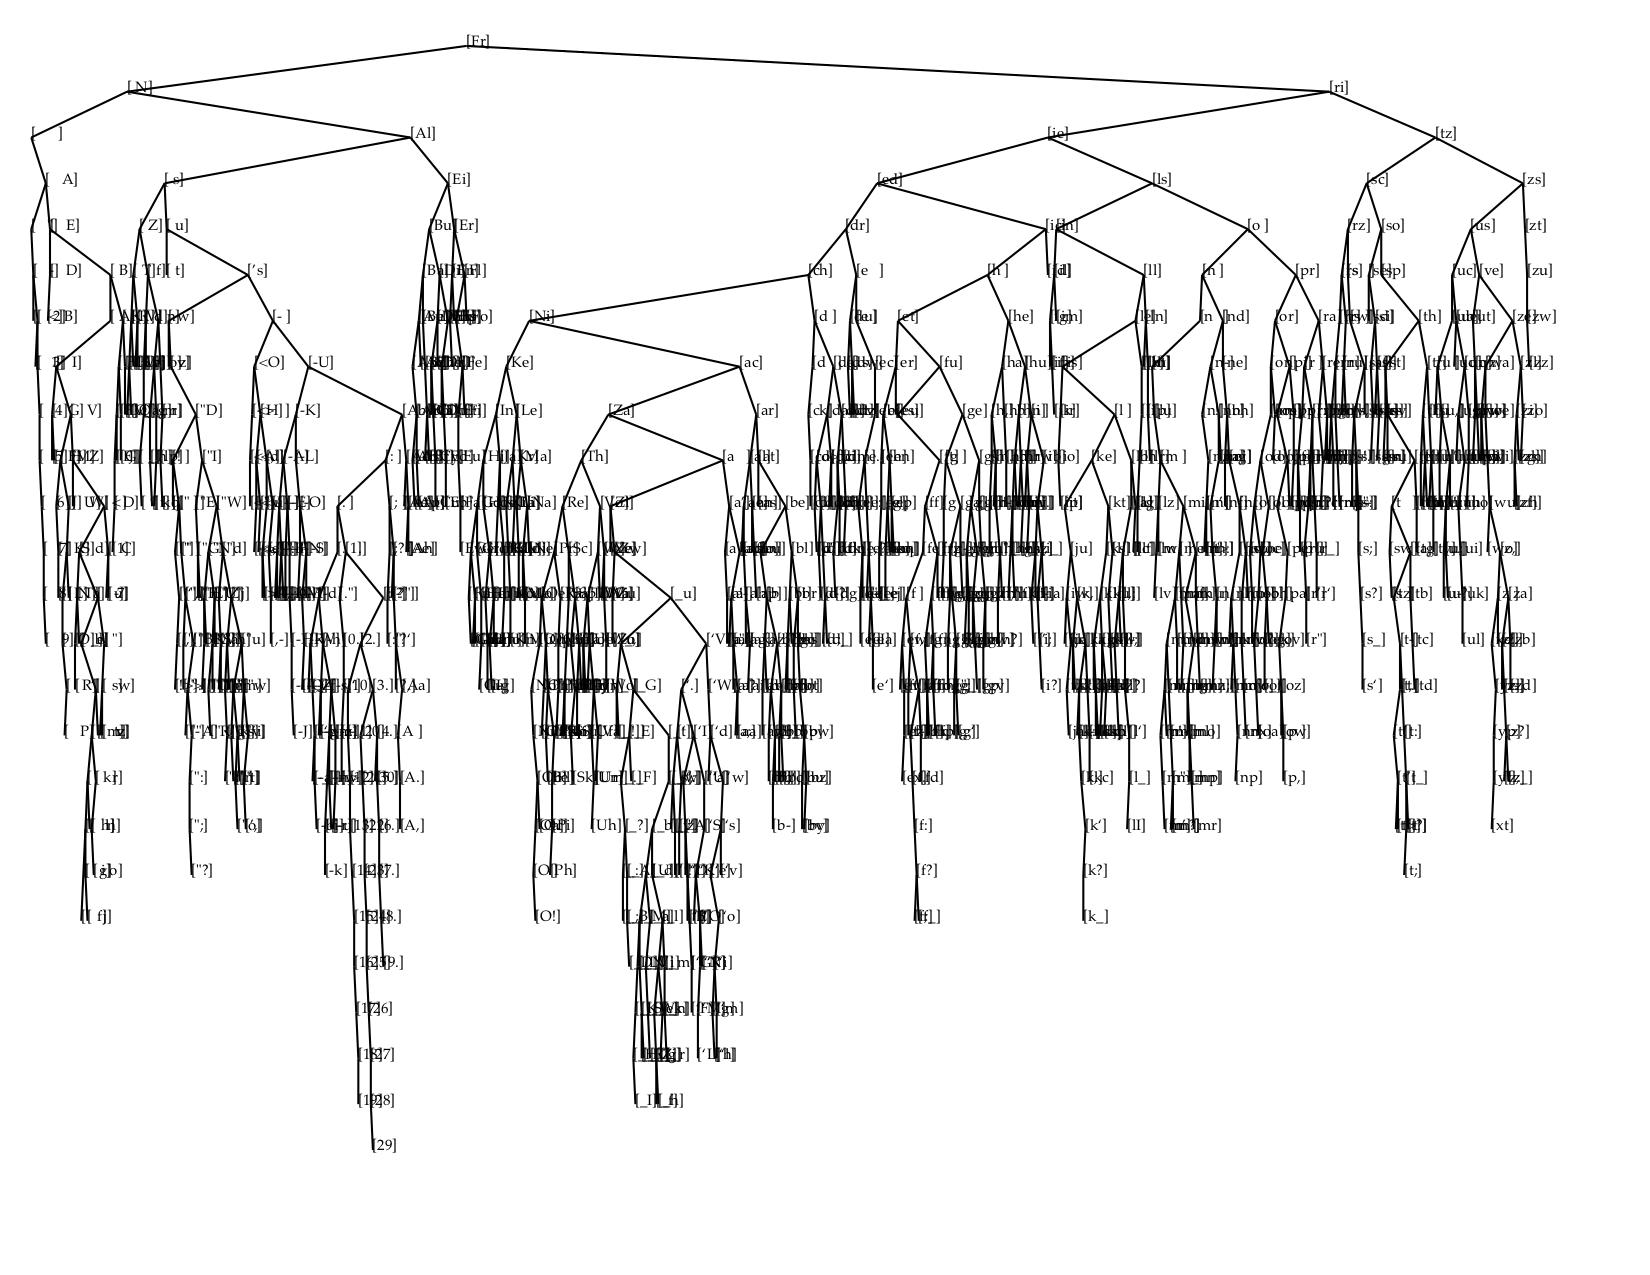
\includegraphics[width=0.99\textwidth]{shakespeareBaum2.png}
\end{center}
\newpage
\mylisting[label=musterloesung1]{Musterlösung}{shakespeare.c}
\mylisting[label=musterloesung2]{Musterlösung}{bintree.c}
\mylisting[label=musterloesung3]{Musterlösung}{bintree.h}
\mylisting[label=musterloesung4]{Musterlösung}{Makefile}

\fi
\end{document}